% 2021 全国乙卷文科第 18 题：四棱锥 P-ABCD，底面矩形，M 为 BC 中点。
% 按指定 PDF 第 1 页（印刷页 1143）重绘；隐藏棱 PD、DA、DC 与辅助线 AM 用虚线。
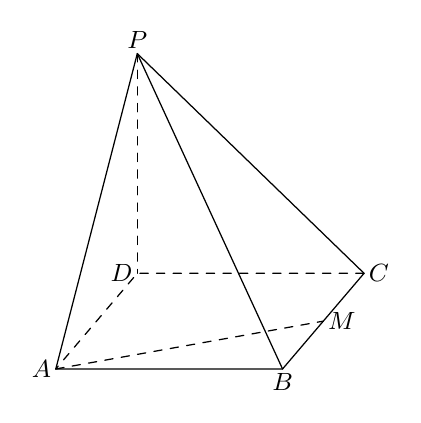
\begin{tikzpicture}[
  x=0.9cm, y=0.9cm,
  font=\small,
  line width=0.45pt,
  line cap=round,
  line join=round,
  every node/.style={inner sep=1.5pt}
]
  \coordinate (A) at (0,0);
  \coordinate (B) at (3.2,0);
  \coordinate (C) at (4.35,1.35);
  \coordinate (D) at (1.15,1.35);
  \coordinate (P) at (1.15,4.45);
  \coordinate (M) at (3.775,0.675);

  % 锥面棱。
  \draw (P) -- (A);
  \draw (P) -- (B);
  \draw (P) -- (C);
  \draw[dashed] (P) -- (D);

  % 矩形底面。
  \draw (A) -- (B) -- (C);
  \draw[dashed] (C) -- (D) -- (A);

  % 题设辅助线 AM。
  \draw[dashed] (A) -- (M);

  \node[anchor=east] at (A) {$A$};
  \node[anchor=north] at (B) {$B$};
  \node[anchor=west] at (C) {$C$};
  \node[anchor=east] at (D) {$D$};
  \node[anchor=south] at (P) {$P$};
  \node[anchor=west] at (M) {$M$};
\end{tikzpicture}
